\chapter{More on certificate authentication}
\index{Certificate authentication}
\label{certificate}

\section{The X.509\index{X.509 certificates} trust model}
\label{x509:trust}

The X.509 protocols rely on a hierarchical trust model. In this trust model
Certification Authorities (CAs) are used to certify entities.
Usually more than one certification authorities exist, and certification
authorities may certify other authorities to issue certificates as well,
following a hierarchical model. 
One needs to trust one or more CAs for his secure
communications. In that case only the certificates issued by the trusted
authorities are acceptable. See figure \ref{fig:x509-1} for a typical example.

\begin{figure}[hbtp]
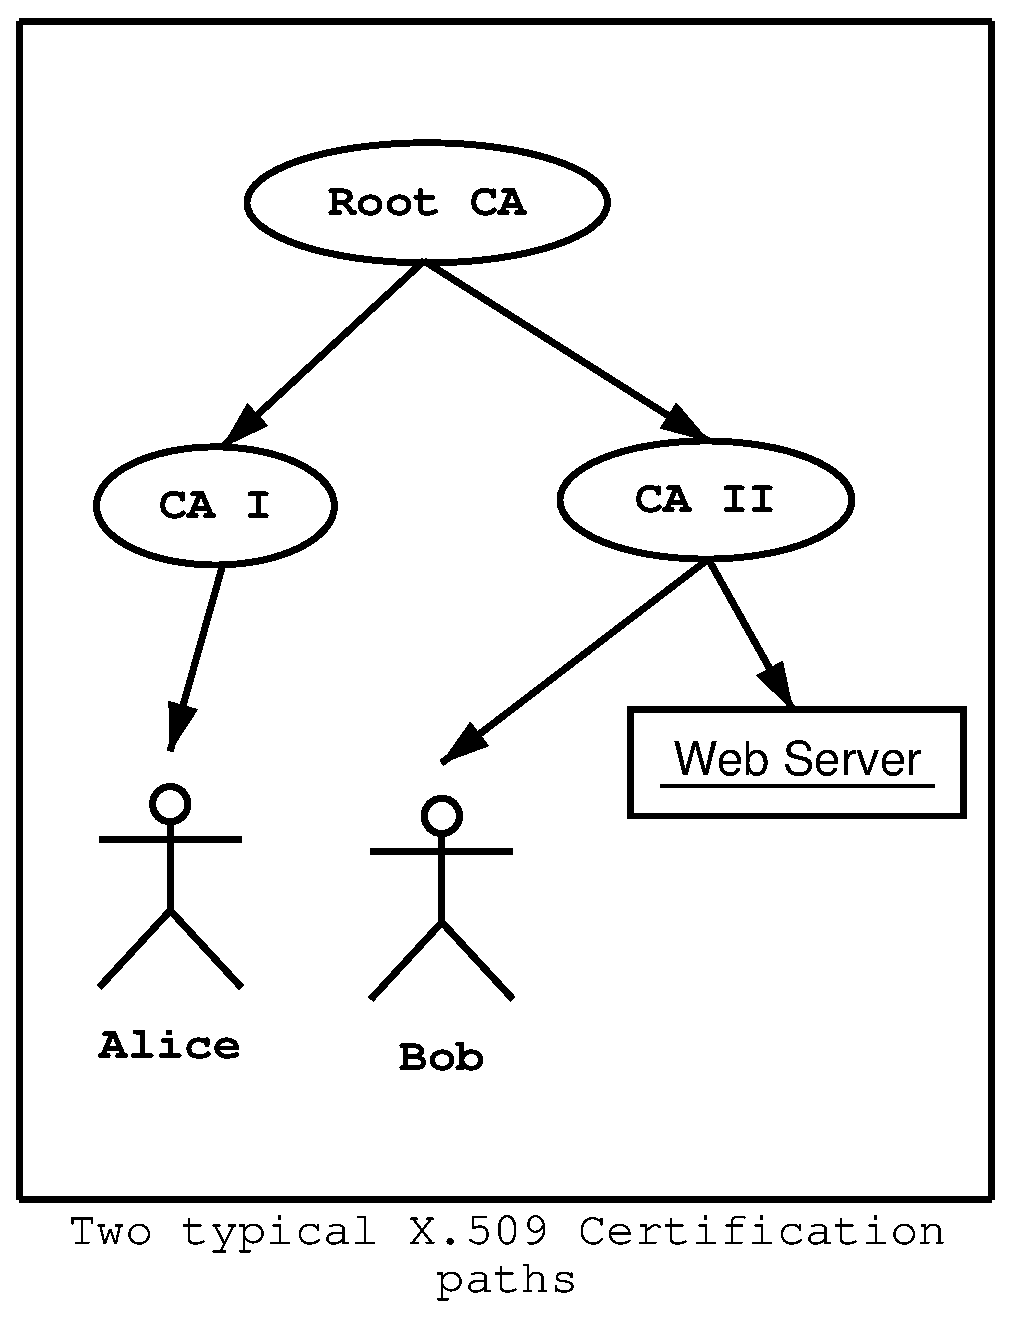
\includegraphics[height=9.5cm,width=9cm]{x509-1}
\label{fig:x509-1}
\end{figure}


The API for handling X.509 certificates is described at section \ref{sec:x509api}
on page \pageref{sec:x509api}. Some examples are listed below.



\subsection{X.509 certificates}
An X.509 certificate usually contains information about the certificate
holder, the signer, a unique serial number, expiration dates etc. Some
functions of \gnutls{}' API for certificate parsing are:
\begin{itemize}
\item \printfunc{gnutls_x509_crt_init}{gnutls\_x509\_crt\_init}
\item \printfunc{gnutls_x509_crt_import}{gnutls\_x509\_crt\_import}
\item \printfunc{gnutls_x509_crt_get_dn}{gnutls\_x509\_crt\_get\_dn}
\item \printfunc{gnutls_x509_crt_get_serial}{gnutls\_x509\_crt\_get\_serial}
\item \printfunc{gnutls_x509_crt_get_subject_alt_name}{gnutls\_x509\_crt\_get\_subject\_alt\_name}
\end{itemize}

\par
An example program that reads the peer's certificate,
and prints some information about the peer's certificate in a TLS session,
is listed below.

\begin{verbatim}

#include <stdio.h>
#include <stdlib.h>
#include <gnutls/gnutls.h>
#include <gnutls/x509.h>

static const char* bin2hex( const void* bin, size_t bin_size)
{
static char printable[110];
unsigned char *_bin = bin;
char* print;

   if (bin_size > 50) bin_size = 50;

   print = printable;
   for (i = 0; i < bin_size; i++) {
      sprintf(print, "%.2x ", _bin[i]);
      print += 2;
   }

   return printable;
}

/* This function will print information about this session's peer
 * certificate. 
 */
static void print_x509_certificate_info(gnutls_session session)
{
   char serial[40];
   char dn[128];
   int i;
   size_t size;
   unsigned int algo, bits;
   time_t expiration_time, activation_time;
   const gnutls_datum *cert_list;
   int cert_list_size = 0;
   gnutls_x509_crt cert;

   /* This function only works for X.509 certificates.
    */
   if (gnutls_certificate_type_get(session) != GNUTLS_CRT_X509)
      return;

   cert_list = gnutls_certificate_get_peers(session, &cert_list_size);

   printf("Peer provided %d certificates.\n", cert_list_size);

   if (cert_list_size > 0) {

      /* we only print information about the first certificate.
       */
      gnutls_x509_crt_init( &cert);

      gnutls_x509_crt_import( cert, &cert_list[0]);

      printf("Certificate info:\n");

      expiration_time = gnutls_x509_crt_get_expiration_time( cert);
      activation_time = gnutls_x509_crt_get_activation_time( cert);

      printf("\tCertificate is valid since: %s", ctime(&activation_time));
      printf("\tCertificate expires: %s", ctime(&expiration_time));

      /* Print the serial number of the certificate.
       */
      size = sizeof(serial);
      gnutls_x509_crt_get_serial(cert, serial, &size);

      size = sizeof( serial);
      printf("\tCertificate serial number: %s\n", 
         bin2hex( serial, size));

      /* Extract some of the public key algorithm's parameters
       */
      algo =
          gnutls_x509_crt_get_pk_algorithm(cert, &bits);

      printf("Certificate public key: ");

      if (algo == GNUTLS_PK_RSA) {
         printf("RSA\n");
         printf(" Modulus: %d bits\n", bits);
      } else if (algo == GNUTLS_PK_DSA) {
         printf("DSA\n");
         printf(" Exponent: %d bits\n", bits);
      } else {
         printf("UNKNOWN\n");
      }

      /* Print the version of the X.509 
       * certificate.
       */
      printf("\tCertificate version: #%d\n",
             gnutls_x509_crt_get_version( cert));

      size = sizeof(dn);
      gnutls_x509_crt_get_dn( cert, dn, &size);
      printf("\tDN: %s\n", dn);

      size = sizeof(dn);
      gnutls_x509_crt_get_issuer_dn( cert, dn, &size);
      printf("\tIssuer's DN: %s\n", dn);

      gnutls_x509_crt_deinit( cert);

   }
}

\end{verbatim}



\subsection{Verifying X.509 certificate paths}
Verifying certificate\index{Verifying certificate paths} paths is important 
in X.509 authentication. For this purpose the function
\printfunc{gnutls_x509_crt_verify}{gnutls\_x509\_crt\_verify} is provided. The
output of this function is the bitwise OR of the elements of the
``gnutls\_certificate\_status'' enumeration. A detailed description of
these elements can be found in figure \ref{fig:verify}.
The function \printfunc{gnutls_certificate_verify_peers}{gnutls\_certificate\_verify\_peers}
is equivalent to the previous one, and will verify the peer's certificate in a TLS session.

\begin{figure}[hbtp]
\begin{tabular}{|l|p{9cm}|}

\hline
CERT\_INVALID & The certificate chain is broken. 
\\
\hline
CERT\_NOT\_TRUSTED & The certificate is not signed by one of the authorities marked as trusted.
\\
\hline
CERT\_REVOKED & The certificate has been revoked.
\\
\hline
CERT\_CORRUPTED & The certificate is corrupted.
\\
\hline
\end{tabular}
\caption{Certificate verification}
\label{fig:verify}
\end{figure}

\par
Although the verification of a certificate path indicates that the
certificate is signed by trusted authority, does not reveal anything
about the peer's identity. It is required to verify if the certificate's
owner is the one you expect. See section \ref{ex:rfc2818} on page \pageref{ex:rfc2818},
for an example.


\subsection{PKCS \#10 certificate requests}
A certificate request is a structure, defined in PKCS \#10, which
is contains information about an applicant of a certificate service.
It usually contains a private key, a distinguished name and secondary
data such as a challenge password.
\par
The following example is about generating a certificate request, and
a private key. A certificate request can be later be processed by a CA,
which should return a signed certificate.

\begin{verbatim}

#include <stdio.h>
#include <stdlib.h>
#include <gnutls/gnutls.h>
#include <gnutls/x509.h>
#include <time.h>

/* This example will generate a private key and a certificate
 * request.
 */

int main()
{
   gnutls_x509_crq_t crq;
   gnutls_x509_privkey_t key;
   unsigned char buffer[10*1024];
   int buffer_size = sizeof(buffer);
   int ret;

   gnutls_global_init();

   /* Initialize an empty certificate request, and
    * an empty private key.
    */
   gnutls_x509_crq_init(&crq);

   gnutls_x509_privkey_init(&key);

   /* Generate a 1024 bit RSA private key.
    */
   gnutls_x509_privkey_generate(key, GNUTLS_PK_RSA, 1024, 0);

   /* Add stuff to the distinguished name
    */
   gnutls_x509_crq_set_dn_by_oid(crq, GNUTLS_OID_X520_COUNTRY_NAME,
				     0, "GR", 2);

   gnutls_x509_crq_set_dn_by_oid(crq, GNUTLS_OID_X520_COMMON_NAME,
				     0, "Nikos", strlen("Nikos"));

   /* Set the request version.
    */
   gnutls_x509_crq_set_version(crq, 1);

   /* Set a challenge password.
    */
   gnutls_x509_crq_set_challenge_password(crq, "something to remember here");

   /* Associate the request with the private key
    */
   gnutls_x509_crq_set_key(crq, key);

   /* Self sign the certificate request.
    */
   gnutls_x509_crq_sign(crq, key);

   /* Export the PEM encoded certificate request, and
    * display it.
    */
   gnutls_x509_crq_export(crq, GNUTLS_X509_FMT_PEM, buffer,
			      &buffer_size);

   printf("Certificate Request: \n%s", buffer);


   /* Export the PEM encoded private key, and
    * display it.
    */
   buffer_size = sizeof(buffer);
   gnutls_x509_privkey_export(key, GNUTLS_X509_FMT_PEM, buffer,
				  &buffer_size);

   printf("\n\nPrivate key: \n%s", buffer);

   gnutls_x509_crq_deinit(crq);
   gnutls_x509_privkey_deinit(key);

   return 0;

}

\end{verbatim}


\subsection{PKCS \#12 structures}
A PKCS \#12 structure usually contains a user's private keys and
certificates. It is commonly used in browsers to export and import
the user's identities.

\par
The following example is about generating a PKCS \#12 structure.

\begin{verbatim}

#include <stdio.h>
#include <stdlib.h>
#include <gnutls/gnutls.h>
#include <gnutls/x509.h>

#define OUTFILE "out.p12"

/* This function will write a pkcs12 structure into a file.
 * cert: is a DER encoded certificate
 * pkcs8_key: is a PKCS #8 encrypted key
 * password: is the password used to encrypt the PKCS #12 packet.
 */
int write_pkcs12(const gnutls_datum * cert, const gnutls_datum * pkcs8_key,
                 const char *password)
{
   gnutls_pkcs12 pkcs12;
   int ret, bag_index;
   gnutls_pkcs12_bag bag, key_bag;
   char pkcs12_struct[10 * 1024];
   int pkcs12_struct_size;
   FILE *fd;

   /* A good idea might be to use gnutls_x509_privkey_get_key_id()
    * to obtain a unique ID.
    */
   gnutls_datum key_id = { "\x00\x00\x00\x01", 4 };

   gnutls_global_init();
   gnutls_global_set_log_level(2);

   /* Firstly we create two helper bags, which hold the certificate,
    * and the (encrypted) key.
    */

   gnutls_pkcs12_bag_init(&bag);
   gnutls_pkcs12_bag_init(&key_bag);

   ret = gnutls_pkcs12_bag_set_data(bag, GNUTLS_BAG_CERTIFICATE, cert);
   if (ret < 0) {
      fprintf(stderr, "ret: %s\n", gnutls_strerror(ret));
      exit(1);
   }

   /* ret now holds the bag's index.
    */
   bag_index = ret;

   /* Associate a friendly name with the given certificate. Used
    * by browsers.
    */
   gnutls_pkcs12_bag_set_friendly_name(bag, bag_index, "My name");

   /* Associate the certificate with the key using a unique key
    * ID.
    */
   gnutls_pkcs12_bag_set_key_id(bag, bag_index, &key_id);

   gnutls_pkcs12_bag_encrypt(bag, password, 0);

   /* Now the key.
    */

   ret = gnutls_pkcs12_bag_set_data(key_bag,
                                    GNUTLS_BAG_PKCS8_ENCRYPTED_KEY,
                                    &pkcs8_key);
   if (ret < 0) {
      fprintf(stderr, "ret: %s\n", gnutls_strerror(ret));
      exit(1);
   }

   /* Note that since the PKCS #8 key is encrypted we don't
    * bother encrypting the bag.
    */
   bag_index = ret;

   gnutls_pkcs12_bag_set_friendly_name(key_bag, bag_index, "My name");

   gnutls_pkcs12_bag_set_key_id(key_bag, bag_index, &key_id);


   /* The bags were filled. Now create the PKCS #12 structure.
    */
   gnutls_pkcs12_init(&pkcs12);

   /* Insert the two bags in the PKCS #12 structure.
    */

   gnutls_pkcs12_set_bag(pkcs12, bag);
   gnutls_pkcs12_set_bag(pkcs12, key_bag);


   /* Generate a message authentication code for the PKCS #12
    * structure.
    */
   gnutls_pkcs12_generate_mac(pkcs12, password);

   pkcs12_struct_size = sizeof(pkcs12_struct);
   ret =
       gnutls_pkcs12_export(pkcs12, GNUTLS_X509_FMT_DER, pkcs12_struct,
                            &pkcs12_struct_size);
   if (ret < 0) {
      fprintf(stderr, "ret: %s\n", gnutls_strerror(size));
      exit(1);
   }

   fd = fopen(OUTFILE, "w");
   if (fd == NULL) {
      fprintf(stderr, "cannot open file\n");
      exit(1);
   }
   fwrite(pkcs12_struct, 1, pkcs12_struct_size, fd);
   fclose(fd);

   gnutls_pkcs12_bag_deinit(bag);
   gnutls_pkcs12_bag_deinit(key_bag);
   gnutls_pkcs12_deinit(pkcs12);

}

\end{verbatim}



\section{The OpenPGP\index{OpenPGP!Keys} trust model}
\label{pgp:trust}

The OpenPGP key authentication relies on a distributed trust model, called
the "web of trust". The "web of trust" uses a decentralized system of 
trusted introducers, which are the same as a CA. OpenPGP allows anyone to 
sign anyone's else public key. When Alice signs Bob's key, she is introducing 
Bob's key to anyone who trusts Alice. If someone trusts Alice to introduce
keys, then Alice is a trusted introducer in the mind of that observer.

\begin{figure}[hbtp]
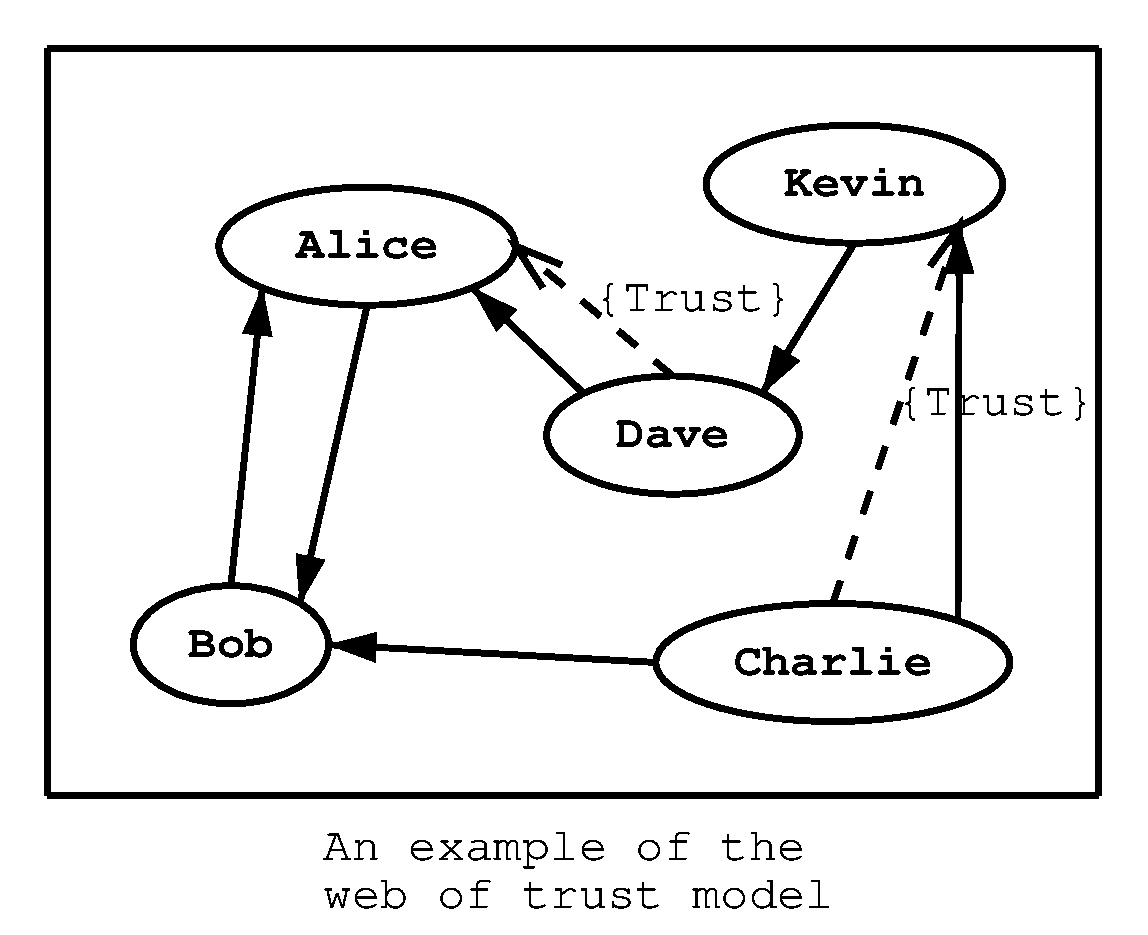
\includegraphics[height=9cm,width=11cm]{pgp-fig1}
\label{fig:pgp1}
\end{figure}

For example: If David trusts Alice to be an introducer, and Alice signed
Bob's key, Dave also trusts Bob's key to be the real one.

There are some key points that are important in that model. In the example
Alice has to sign Bob's key, only if she is sure that the key belongs
to Bob. Otherwise she may also make Dave falsely believe that this
is Bob's key. Dave has also the responsibility to know who to trust.
This model is similar to real life relations.

Just see how Charlie behaves in the previous example. Although he has 
signed Bob's key - because he knows, somehow, that it belongs to Bob - 
he does not trust Bob to be an introducer. Charlie decided to trust only 
Kevin, for some reason. A reason could be that Bob is lazy enough, and 
signs other people's keys without being sure that they belong to the 
actual owner.

\subsection{Verifying an OpenPGP key}
First we've to differentiate between ownertrust and validity. Sometimes trust
and validity is used as a synonym but this is not correct.
\par
The ownertrust describes how trustworthy the signature of a special
key owner is. Even if we've three or more signatures to make a key valid,
it's possible that we don't trust the owner at all and thus we don't trust 
the signature he made. There are different ownertrust levels:
\begin{enumerate}
\item Don't know
\item I do NOT trust
\item I trust marginally
\item I trust fully
\item I trust ultimately.
\end{enumerate}

For example we need three marginally trusted signature to make a key
valid or one full trusted signature. The ultimate trust is only used
when we are the owner of a key and we also have the secret key.
In the case we don't trust the owner, those signatures are skipped
for the web of trust calculation.
\par
All checks in GnuTLS are done in \printfunc{gnutls_openpgp_verify_key}{gnutls\_openpgp\_verify\_key}. 
If a trust database is available, this is the file which contains all information about the
key owner (ownertrust), additional checks are performed.
\\
First we get the trustdb entry to see if the key is not disabled because
those keys shouldn't be used at all. Another possible case is that we
don't trust the key, which means we don't need to perform further checks.
\par
If the ownertrust is at least marginal we continue to check all signatures
the key contains to get the validity of the key. It is likely that the
public keyring does not contain all needed keys to check all signatures.
When a signature could not be checked due to a missing key, the function 
tries the next signature. When NO public key is available, the function
checks at least the self signature which must be valid in any case because
it was created by the key itself.
\\
Validity means if the signatures on the key are valid and the key was not 
changed by somebody or corrupted during transport.

